\documentclass[11pt]{article}
\usepackage{amsmath, amssymb}
\usepackage{anysize,color,graphicx,url,hyperref}
\usepackage{xcolor}
\usepackage{HW}

\hypersetup{
    colorlinks=true,
    linkcolor=blue,
    filecolor=magenta,
    urlcolor=red,
}

\graphicspath{{images/}}
\marginsize{1in}{1in}{1in}{1in}

\title{Task 02: Single View Geometry and Distance Estimation}
\author{}
\date{\today}

\begin{document}
\maketitle

\section*{Honor Code and Disclosure}

I have attempted this assignment honestly and have not intentionally misrepresented any result. A large language model was used to help set up the native Apple Silicon environment, organize the scripts, run the code, and explain the method with a human in the loop checking the outputs and deciding what assumptions were acceptable. The LLM was not used as a substitute for understanding the geometry. The important human-checked assumptions are listed explicitly below: the Google Maps reference distance, the image points on the blue line, and the choice of bottom-center of the detection box as the object reference point.

External sources and tools used:
\begin{itemize}
    \item Google Maps Measure Distance tool for the real-world reference distance.
    \item Ultralytics YOLO documentation: \url{https://docs.ultralytics.com/quickstart}
    \item PyTorch local install documentation: \url{https://pytorch.org/get-started/locally/}
    \item PyTorch MPS backend documentation: \url{https://docs.pytorch.org/docs/2.12/notes/mps.html}
    \item Apple Metal PyTorch documentation: \url{https://developer.apple.com/metal/pytorch/}
\end{itemize}

\section{Who Moved My Bicycle?}

\subsection{Final Distance Estimate}

For the provided IIT Bombay image, my estimated real-world distance between the bicycle and the arch is approximately
\[
\boxed{117\ \text{m}}
\]
using the bottom-center of the YOLO bicycle bounding box as the bicycle's ground-contact point. The corresponding estimated distance from the MB red line to the bicycle is approximately
\[
43\ \text{m}.
\]
These values are approximate because the image points are manually selected on a perspective image.

\subsection{Google Maps Reference Distance}

I used Google Maps' Measure Distance tool to estimate the real-world distance from the MB red line location to the IIT Bombay arch. Rounded to the nearest multiple of 10 metres, I used
\[
AC = 160\ \text{m}.
\]
Here \(A\) is the real-world position corresponding to the red MB line and \(C\) is the real-world position corresponding to the arch along the MB-to-arch road direction.

\subsection{Why Google Maps Cannot Directly Give the Bicycle Distance}

Google Maps cannot directly give the bicycle distance because the bicycle is only an object visible in a perspective photograph, not a named map location with known GPS coordinates.

\subsection{Annotated Cross-Ratio Line}

I drew one dark-blue line along the visible road direction from the red MB line toward the arch. The four image points used for cross-ratio were placed on this same line:
\begin{itemize}
    \item \(A'\): where the dark-blue road line meets the red MB line.
    \item \(B'\): the bicycle point, chosen as the bottom-center of the YOLO bounding box.
    \item \(C'\): the arch point on the same road line.
    \item \(V'\): the vanishing point of the road direction.
\end{itemize}

\begin{figure}[h!]
\centering
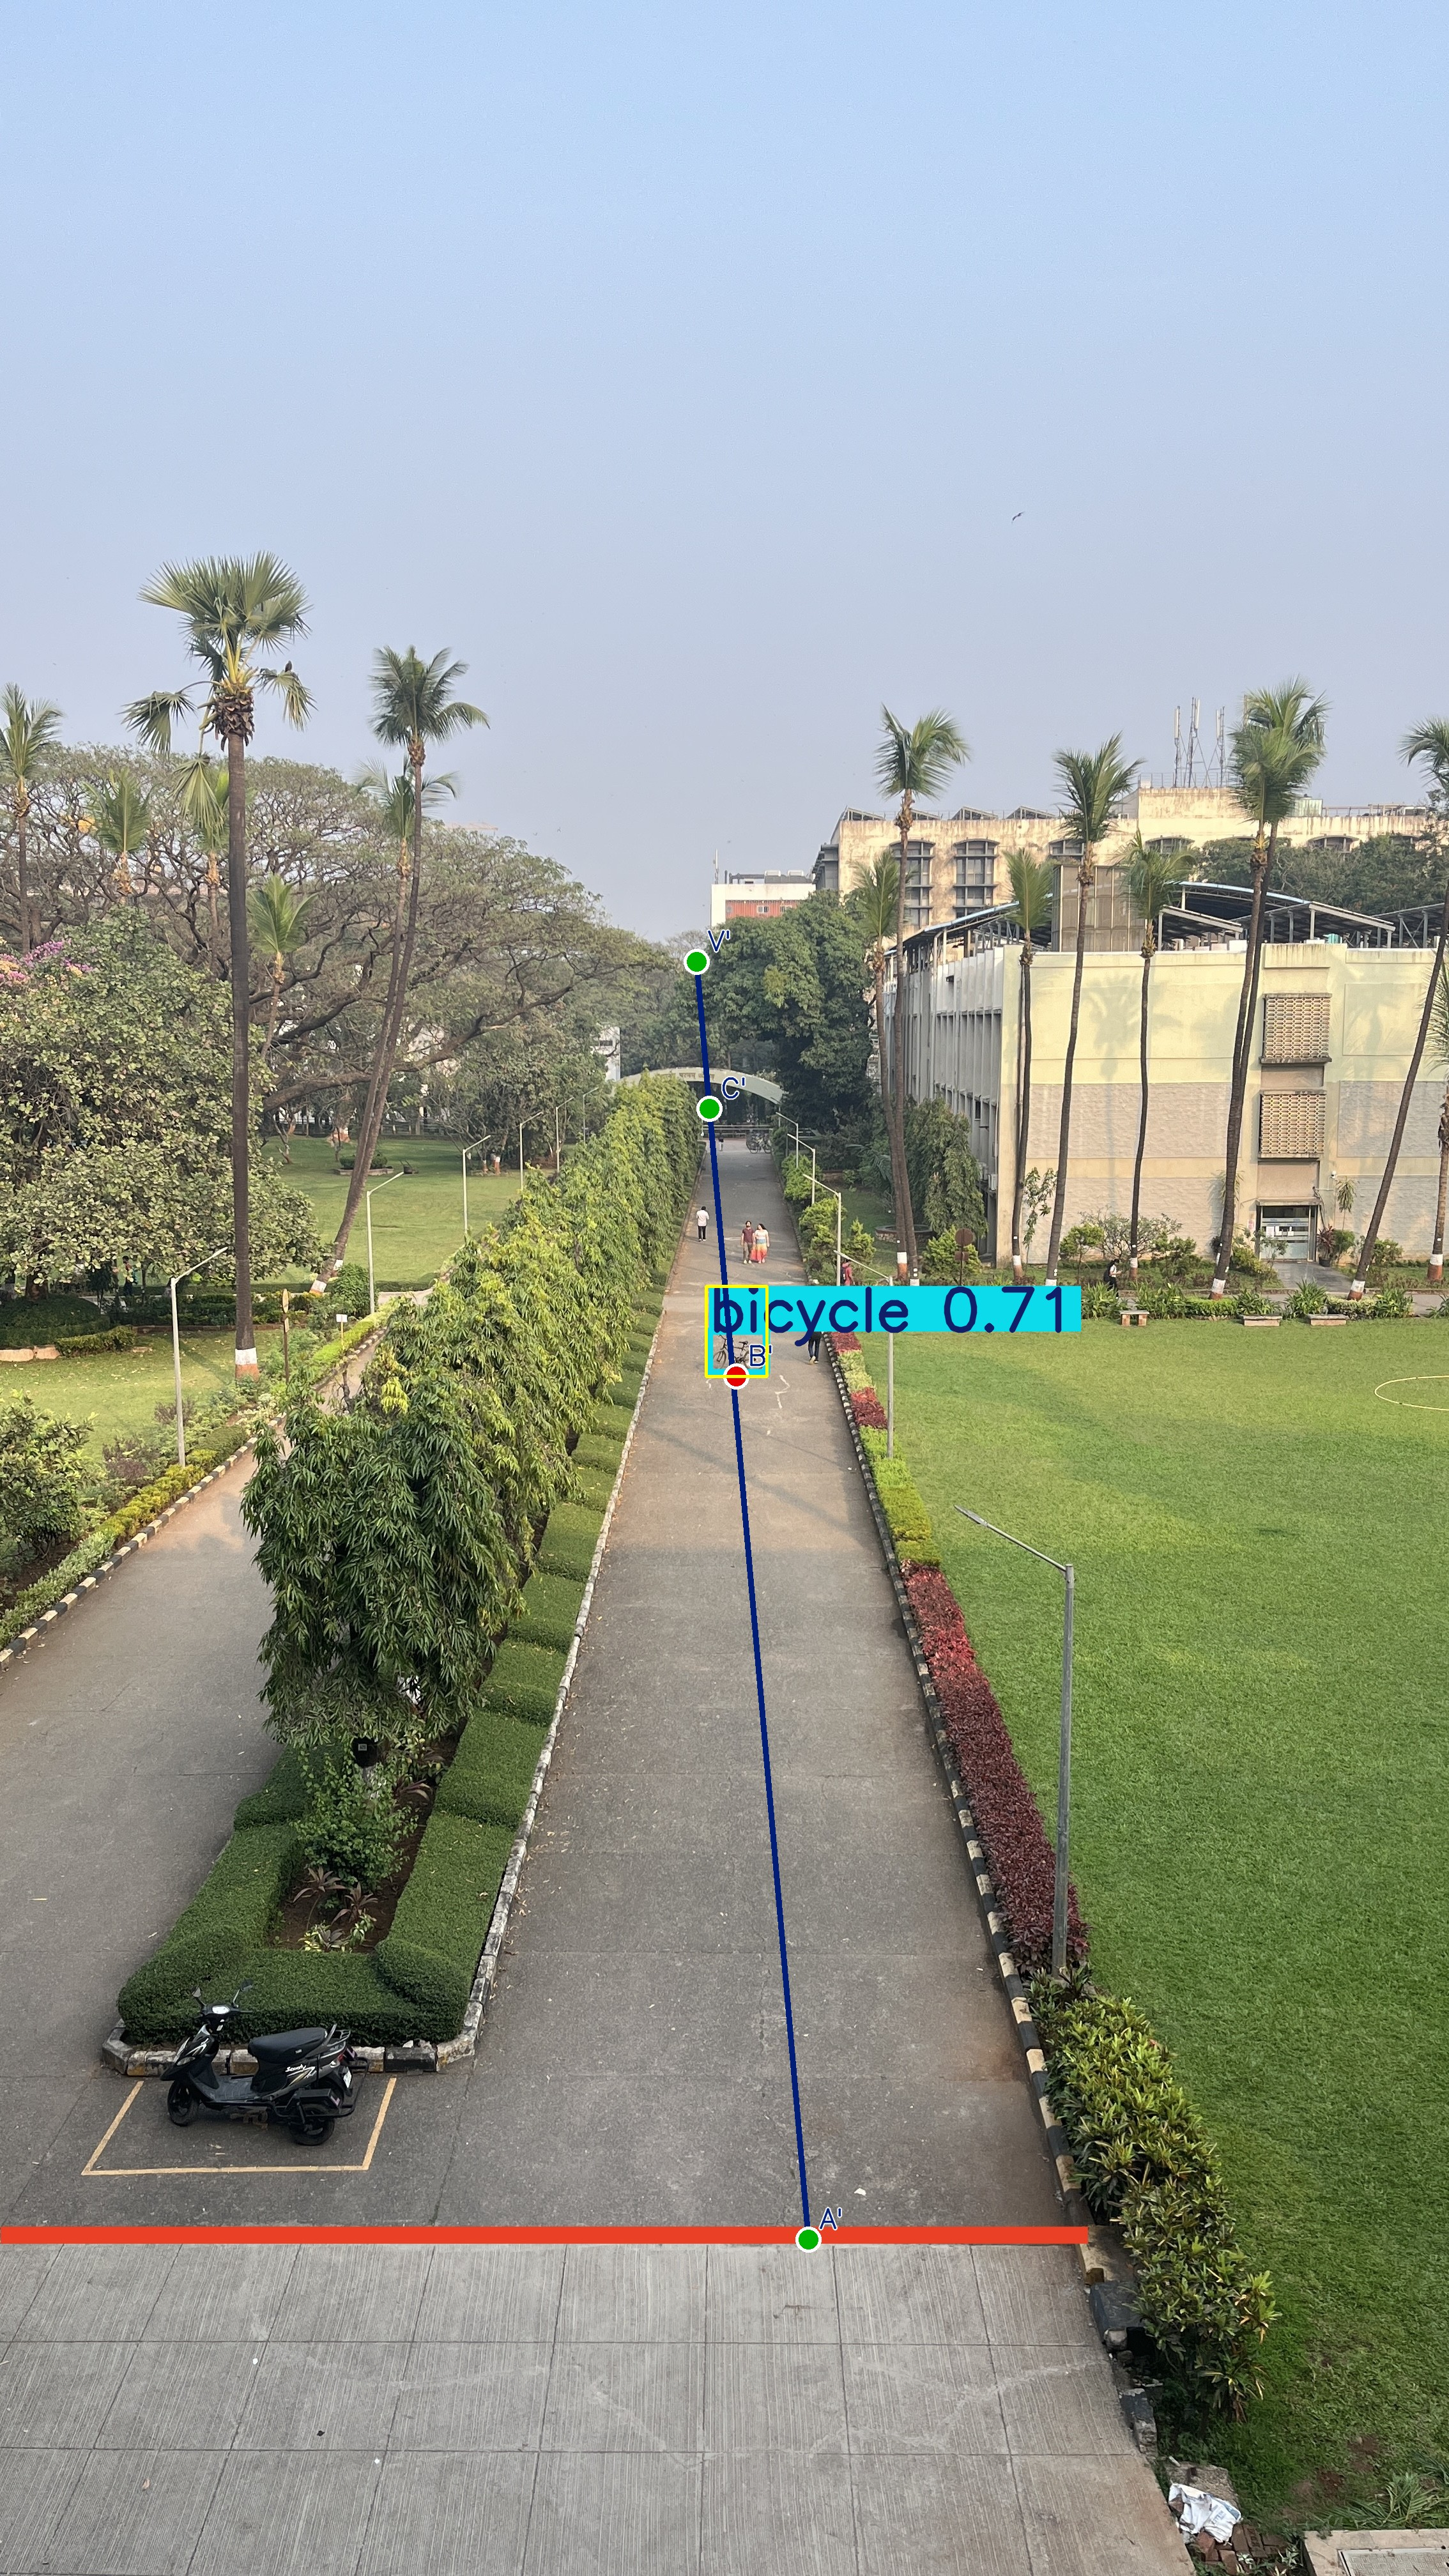
\includegraphics[width=0.62\linewidth]{cross_ratio_annotation.jpg}
\caption{Annotated image with the dark-blue 1D projective line and points \(A'\), \(B'\), \(C'\), \(V'\).}
\end{figure}

This collinearity is important because cross-ratio is a one-dimensional projective invariant. If the four points are not on the same image line, then the computation would no longer match the theory being used.

\subsection{Meaning of A' and B'}

The point \(A'\) corresponds to the red MB reference line in the image, i.e. the start point of the measured real-world road segment. The point \(B'\) corresponds to the bicycle's estimated ground contact point. I used the bottom-center of the YOLO bounding box because distance is being measured along the ground plane, and the lower edge of the object box is closer to the object's contact with the ground than the visual center of the box.

\subsection{Method and Code}

The method has two parts: object localization and projective distance estimation.

For object localization, I used an Ultralytics YOLO model. COCO class id \(1\) is the bicycle class and COCO class id \(0\) is the person class. The script \texttt{scripts/detect\_yolo.py} loads a pretrained YOLO model, runs prediction on the image, filters by the requested class id, and writes a JSON file containing bounding boxes. The relevant output fields are the box coordinates \((x_1,y_1,x_2,y_2)\), the center, and the bottom-center point. For the assignment image, the provided figure already contains a YOLOv8 bicycle prediction. When I ran YOLO on this already annotated PNG, the turquoise label partially covered the bicycle, so the model did not rediscover the bicycle reliably from the modified image. Therefore, for the provided image I used the visible YOLO bicycle box already present in the assignment figure:
\[
(x_1,y_1,x_2,y_2) = (1105, 2013, 1200, 2154).
\]
The bottom-center bicycle point is therefore approximately
\[
B' = \left(\frac{1105+1200}{2}, 2154\right) = (1152.5, 2154).
\]

For distance estimation, I used the script \texttt{scripts/estimate\_cross\_ratio.py}. The manually selected image points are stored in \texttt{points/bicycle\_points.json}:
\[
A'=(1265,3505),\quad C'=(1110,1735),\quad V'=(1090,1505).
\]
The script projects each 2D point onto the selected blue image line so that the calculation becomes one-dimensional. It then computes
\[
\operatorname{CR}(A',B';C',V')
=
\frac{(C'-A')/(C'-B')}{(V'-A')/(V'-B')}.
\]
In the real world, \(V\) is the point at infinity along the road direction. With \(A=0\) and \(C=160\) m, the corresponding real-world relation becomes
\[
\operatorname{CR}(A,B;C,V)=\frac{AC}{AC-AB}.
\]
Solving for \(AB\),
\[
AB = AC\left(1-\frac{1}{\operatorname{CR}}\right).
\]
Then the bicycle-to-arch distance is
\[
BC = AC - AB.
\]

Using the bottom-center point, the script reported
\[
AB = 43.23\ \text{m},\qquad BC = 116.77\ \text{m}.
\]
So I report the bicycle-to-arch distance as approximately \(117\) m.

\subsection{Effect of Bounding-Box Reference Point}

The choice of reference point inside the bounding box does affect the result. The reason is that a small vertical movement in the image can represent a large movement along the ground plane under perspective projection. The script tested several possible points inside the same bounding box:

\begin{center}
\begin{tabular}{lrr}
\hline
Reference point & MB to bicycle (m) & Bicycle to arch (m) \\
\hline
Bottom-center & 43.23 & 116.77 \\
Bottom-left & 43.64 & 116.36 \\
Bottom-right & 42.82 & 117.18 \\
Center & 50.96 & 109.04 \\
Top-center & 60.81 & 99.19 \\
\hline
\end{tabular}
\end{center}

The bottom-left and bottom-right choices differ by less than \(1\) m in the bicycle-to-arch result, while top-center changes the bicycle-to-arch estimate by about \(17.58\) m compared with bottom-center. This confirms that vertical reference point selection is a major source of error. I chose bottom-center because it is the most geometrically meaningful point for an object standing or resting on the ground.

\section{Native Apple Silicon Environment}

The code was run in a single native Apple Silicon conda environment named \texttt{coolalgo}. An older mixed-architecture \texttt{coolalgo} environment was removed so that the assignment used one native environment only. The verified native setup was:
\begin{itemize}
    \item Python architecture: \texttt{arm64}
    \item OpenCV binary: \texttt{arm64}
    \item PyTorch version: \texttt{2.12.0}
    \item Ultralytics version: \texttt{8.4.67}
    \item MPS available outside the command sandbox: \texttt{True}
\end{itemize}
The YOLO script was also verified using \texttt{--device mps}, and it printed \texttt{using device: mps}. The projective geometry script does not need the GPU; it uses NumPy and OpenCV for arithmetic and annotation.

\section{Your Picture}

\subsection{Captured Images}

I captured the required two images indoors. The first-person view image is the main image used for detecting the teammate/person. The third-person view image records the setup and shows the camera holder and the person being photographed.

\begin{figure}[h!]
\centering
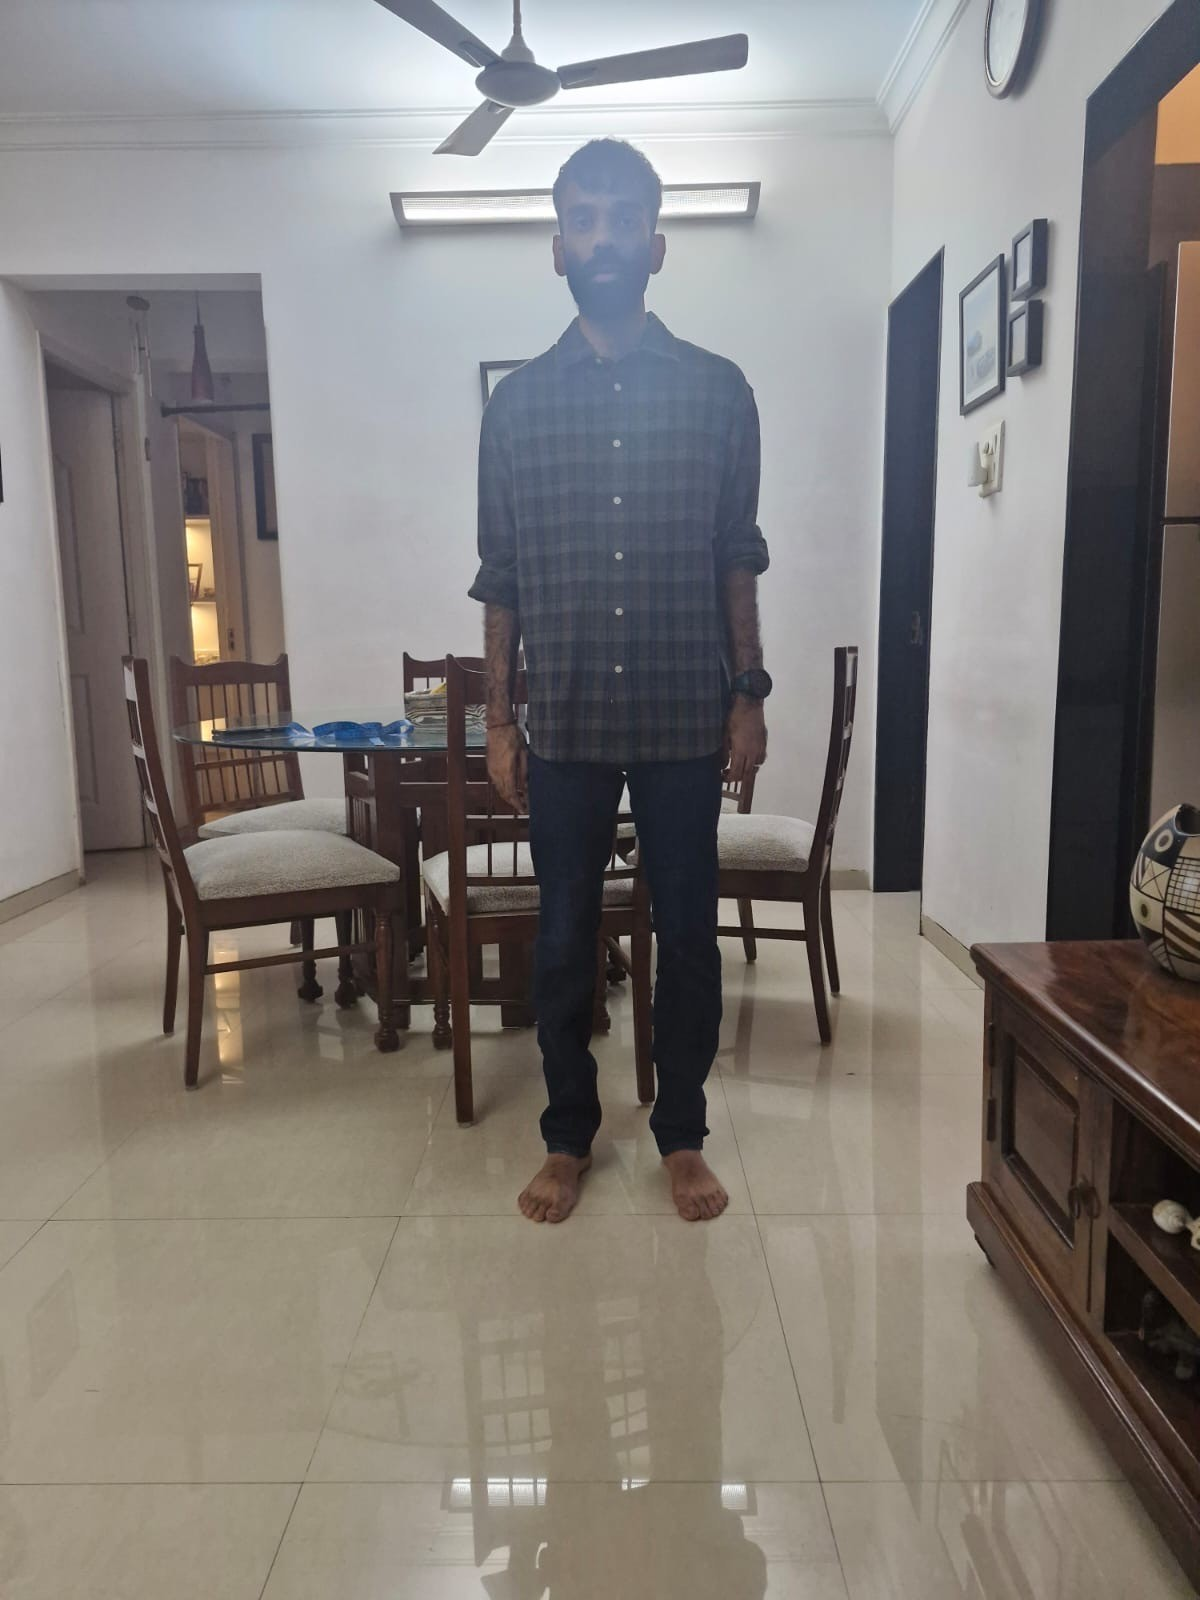
\includegraphics[width=0.45\linewidth]{firstPersonView_display.jpg}
\caption{First-person view image used for person detection.}
\end{figure}

\begin{figure}[h!]
\centering
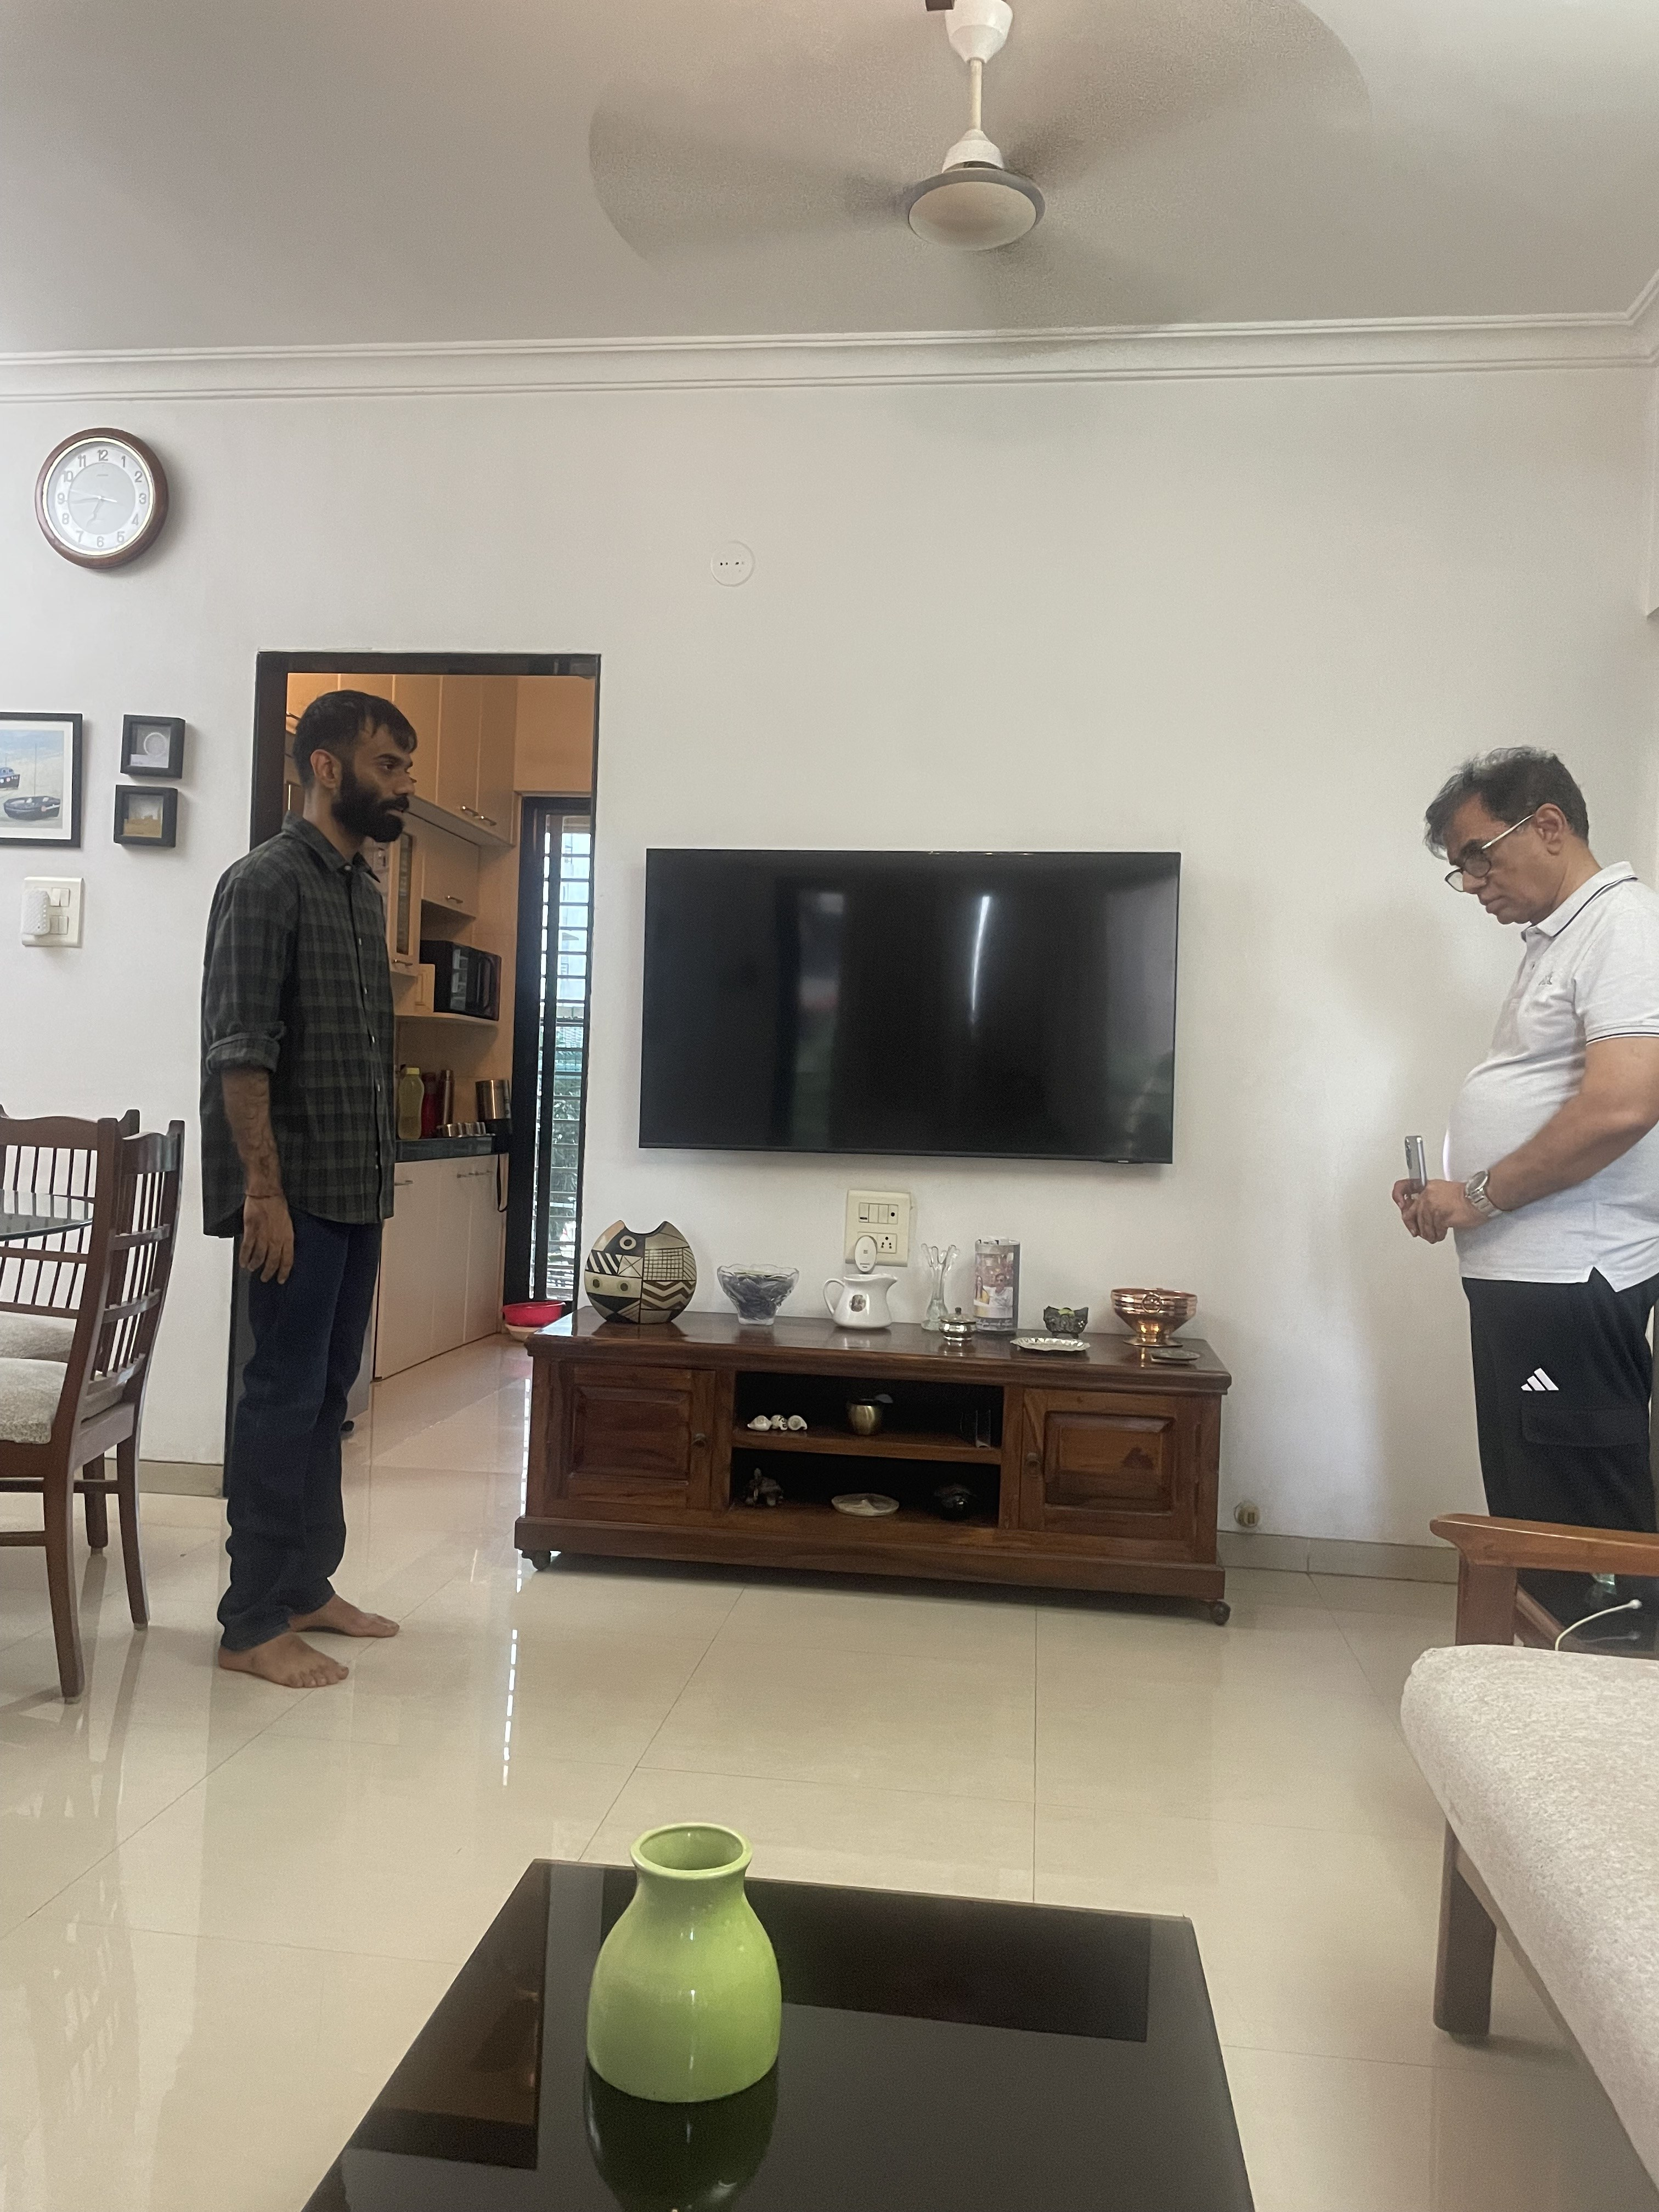
\includegraphics[width=0.62\linewidth]{thirdPersonView_display.jpg}
\caption{Third-person view image showing the image capture setup.}
\end{figure}

\subsection{Person Detection}

I used the same YOLO script as before, but with COCO class id \(0\), which corresponds to the \texttt{person} class. The command used was:
\[
\texttt{python scripts/detect\_yolo.py images/firstPersonView.jpeg --class-id 0 --device mps}
\]
The model detected one person in the first-person image:
\[
(x_1,y_1,x_2,y_2)=(465.8,139.2,773.8,1233.4),
\]
with confidence \(0.904\). The bottom-center point of the detected person box is therefore approximately
\[
B'=\left(\frac{465.8+773.8}{2},1233.4\right)=(619.8,1233.4).
\]

\begin{figure}[h!]
\centering
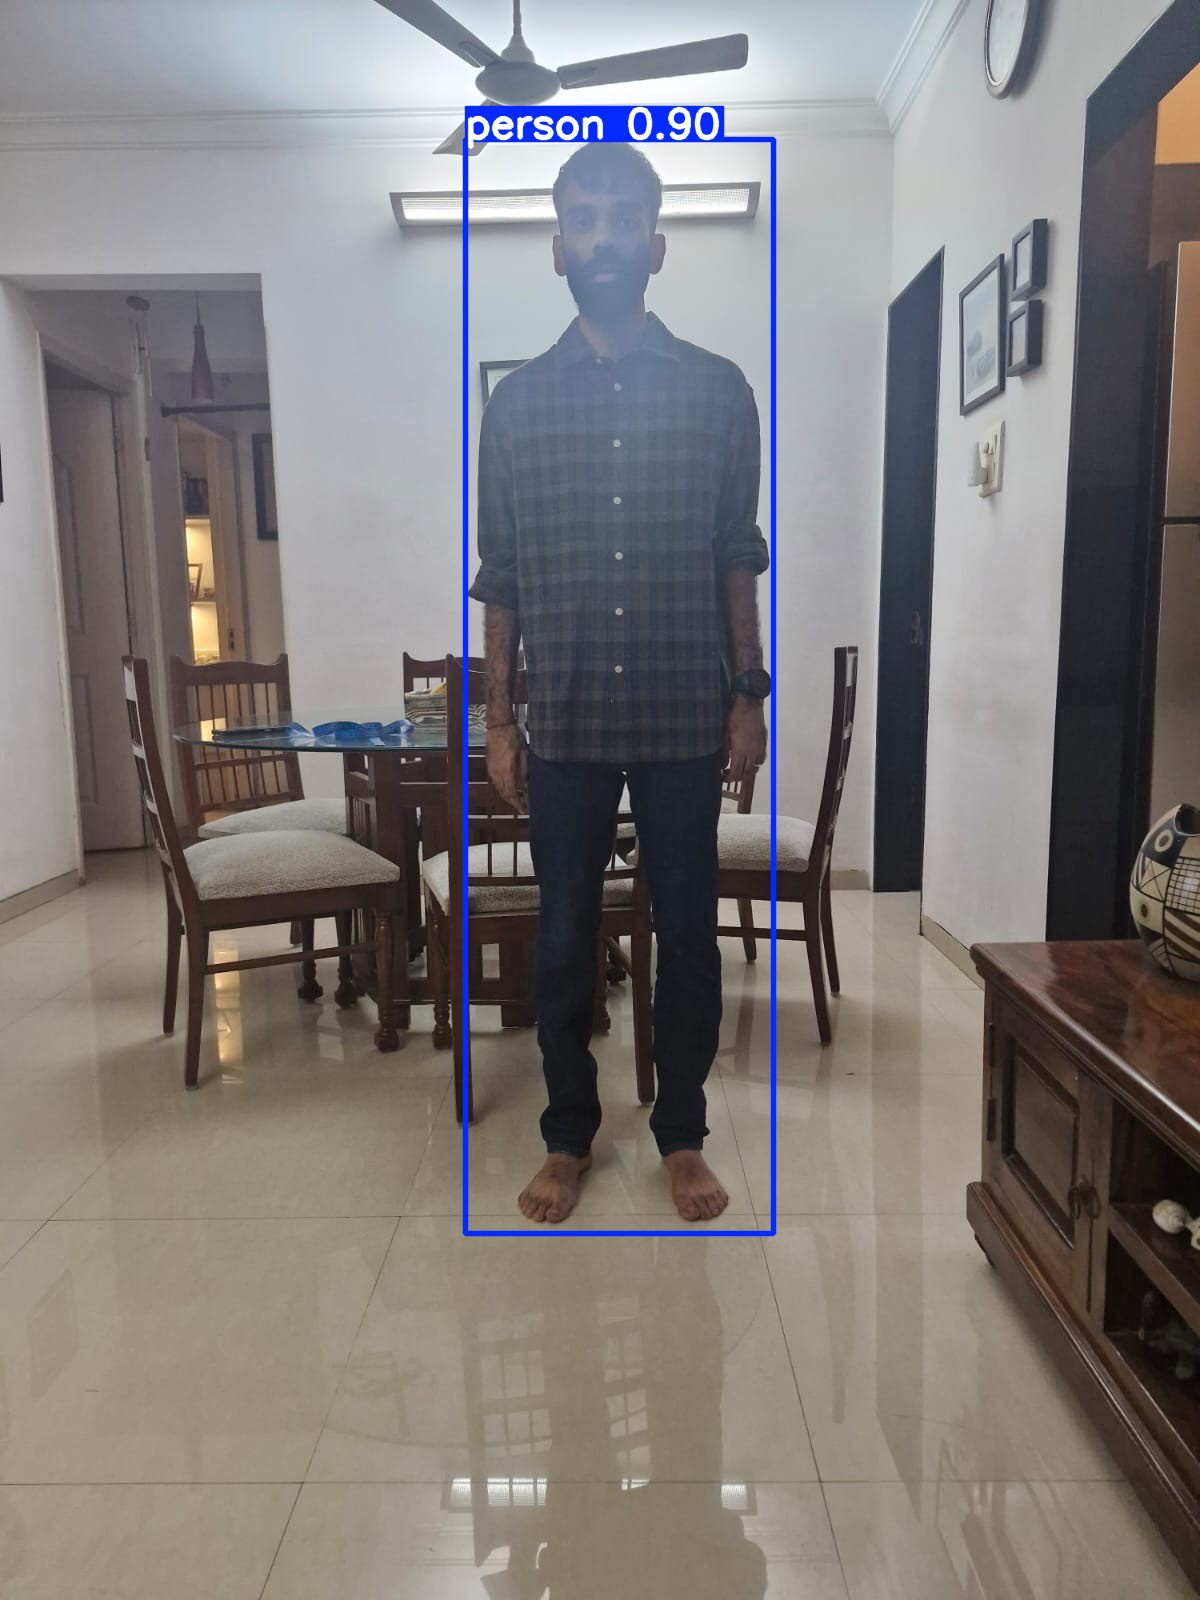
\includegraphics[width=0.45\linewidth]{firstPersonView_yolo_class0.jpg}
\caption{YOLO person detection on the first-person image.}
\end{figure}

\subsection{Distance Estimate for My Picture}

For this personal-photo experiment, the camera-to-person distance was physically measured as \(6\) feet. Converting to metres:
\[
6\ \text{ft}\times 0.3048 = 1.8288\ \text{m}.
\]
So the reported camera-to-person distance is
\[
\boxed{1.83\ \text{m}}
\]
or equivalently \(6\) feet.

This personal image was taken indoors, where a direct physical measurement was available. Therefore, unlike the bicycle image, the most reliable distance estimate for the person is the measured distance. I still used YOLO to satisfy the object-detection part of the task and to locate the person in the image. If a longer indoor corridor or outdoor path had been used, I would repeat the full cross-ratio method by selecting \(A'\), \(B'\), \(C'\), and \(V'\) on one floor/road line and using a known measured \(AC\) reference distance.

\subsection{Line of Interest and Points}

In this indoor image, the floor tile seams provide visible straight-line cues, but the person is close to the camera and the directly measured camera-to-person distance is more reliable than estimating the same quantity using a manually selected vanishing point. I therefore used the physical camera-to-person measurement as the real-world distance and used YOLO only to detect the person. The relevant image point for the person is \(B'\), the bottom-center of the detected person box, because that is closest to where the feet touch the ground plane.

For a full cross-ratio version of the same scene, the steps would be:
\begin{enumerate}
    \item choose a near floor point \(A'\) and a farther floor point \(C'\) on the same tile seam,
    \item measure the real-world distance \(AC\),
    \item mark \(V'\), the vanishing point of that tile seam direction,
    \item use the detected bottom-center person point as \(B'\),
    \item run the same cross-ratio script used for the bicycle image.
\end{enumerate}

\subsection{Expected Practical Challenges}

The practical challenges encountered or observed are:
\begin{enumerate}
    \item \textbf{Choosing collinear points:} The cross-ratio formula only makes sense when \(A'\), \(B'\), \(C'\), and \(V'\) lie on one image line. In a real photo, the correct road direction may be visually ambiguous.
    \item \textbf{Vanishing point sensitivity:} A small change in \(V'\) can move the result by several metres, especially when the vanishing point is close to the reference point in the image.
    \item \textbf{Bounding-box ground contact:} YOLO returns a rectangular box, not the exact foot or wheel contact point. Choosing the center of the box instead of bottom-center creates a significant distance error.
    \item \textbf{Reference measurement mismatch:} The real-world distance measured in Google Maps must correspond to the exact segment used in the image. If the map points and image points are not the same physical points, the scale is wrong.
    \item \textbf{Occlusion and image quality:} Object detection can fail if the object is partly covered, too small, blurry, or already covered by an annotation label.
    \item \textbf{Indoor scene limitations:} In the personal photo, the person is close to the camera and the room does not provide a long road-like depth line. Direct physical measurement is therefore more trustworthy than forcing a fragile cross-ratio estimate.
\end{enumerate}

\subsection{Programs Written}

I wrote two main programs:
\begin{itemize}
    \item \texttt{scripts/detect\_yolo.py}: runs YOLO object detection, supports COCO class filtering, saves detection JSON, saves an annotated detection image, and automatically uses Apple \texttt{mps} when available.
    \item \texttt{scripts/estimate\_cross\_ratio.py}: reads a JSON file of image points and the reference distance, projects points onto a single line, computes the cross-ratio distance estimate, tests several bounding-box reference points, and saves the annotated blue-line image.
\end{itemize}

I also used \texttt{points/bicycle\_points.json} to keep the point selections reproducible instead of hiding them inside the code.

\end{document}
